\documentclass[12pt]{article}
\usepackage{amsmath}
\usepackage{babel}
\usepackage{graphicx}
\usepackage{subcaption}
\usepackage{upgreek}
\usepackage[section]{placeins}
\usepackage{subcaption}
\usepackage{amssymb}
\usepackage{amsmath}
\usepackage{xepersian}
\settextfont {XB Zar.TTF}
\let\oldnorm\norm   % <-- Store original \norm as \oldnorm
\let\norm\undefined % <-- "Undefine" \norm
\DeclarePairedDelimiter\norm{\lVert}{\rVert}
\title{پروژه فصلی ۲ : بررسی مدار سفر از زمین به مریخ}
\author{حسین حاتم نیا ۹۸۱۱۰۱۹۲ - ارمیا اعتمادی بروجنی 98100594}
\date{}

\begin{document}
	\maketitle
	\section*{مقدمه}
	در این پروژه سفر یک فضاپیما از زمین به مریخ را بررسی می‌کنیم و مشخصات مداری، زمان سفر و سرعت در هر مرحله را محاسبه می‌کنیم. در ادامه سوخت مورد نیاز و زمانی که لازم است برای پرتاب لازم است را بدست می‌اوریم. نتایج عددی در \lr{Python }  به کمک روش اویلر محاسبه شده و برای نمایش نتایج از \lr{Matplotlib} و \lr{vPython} استفاده شده. 
	\section*{بررسی اولیه مسئله : مدار هوهمان}
	برای رفتن از مدار زمین به مدار مریخ یکی از معروف‌‌ترین مسیر ها، "مدار هوهمان" هست. در مدار هوهمان یک مدار بیضی با حضیض در فاصله مدار کوچکتر و اوج در فاصله مدار بزرگتر تشکیل می‌دهیم. این مدار در این دو نقطه به مدار دو سیاره مماس است. پس با اعمال دو مرحله پیشرانه و افزایش سرعت می‌توان به کمک مدار هوهمان این سفر را انجام داد. شکل تقریبی مدار و محاسبات اولیه در ادامه آمده اند:
	
	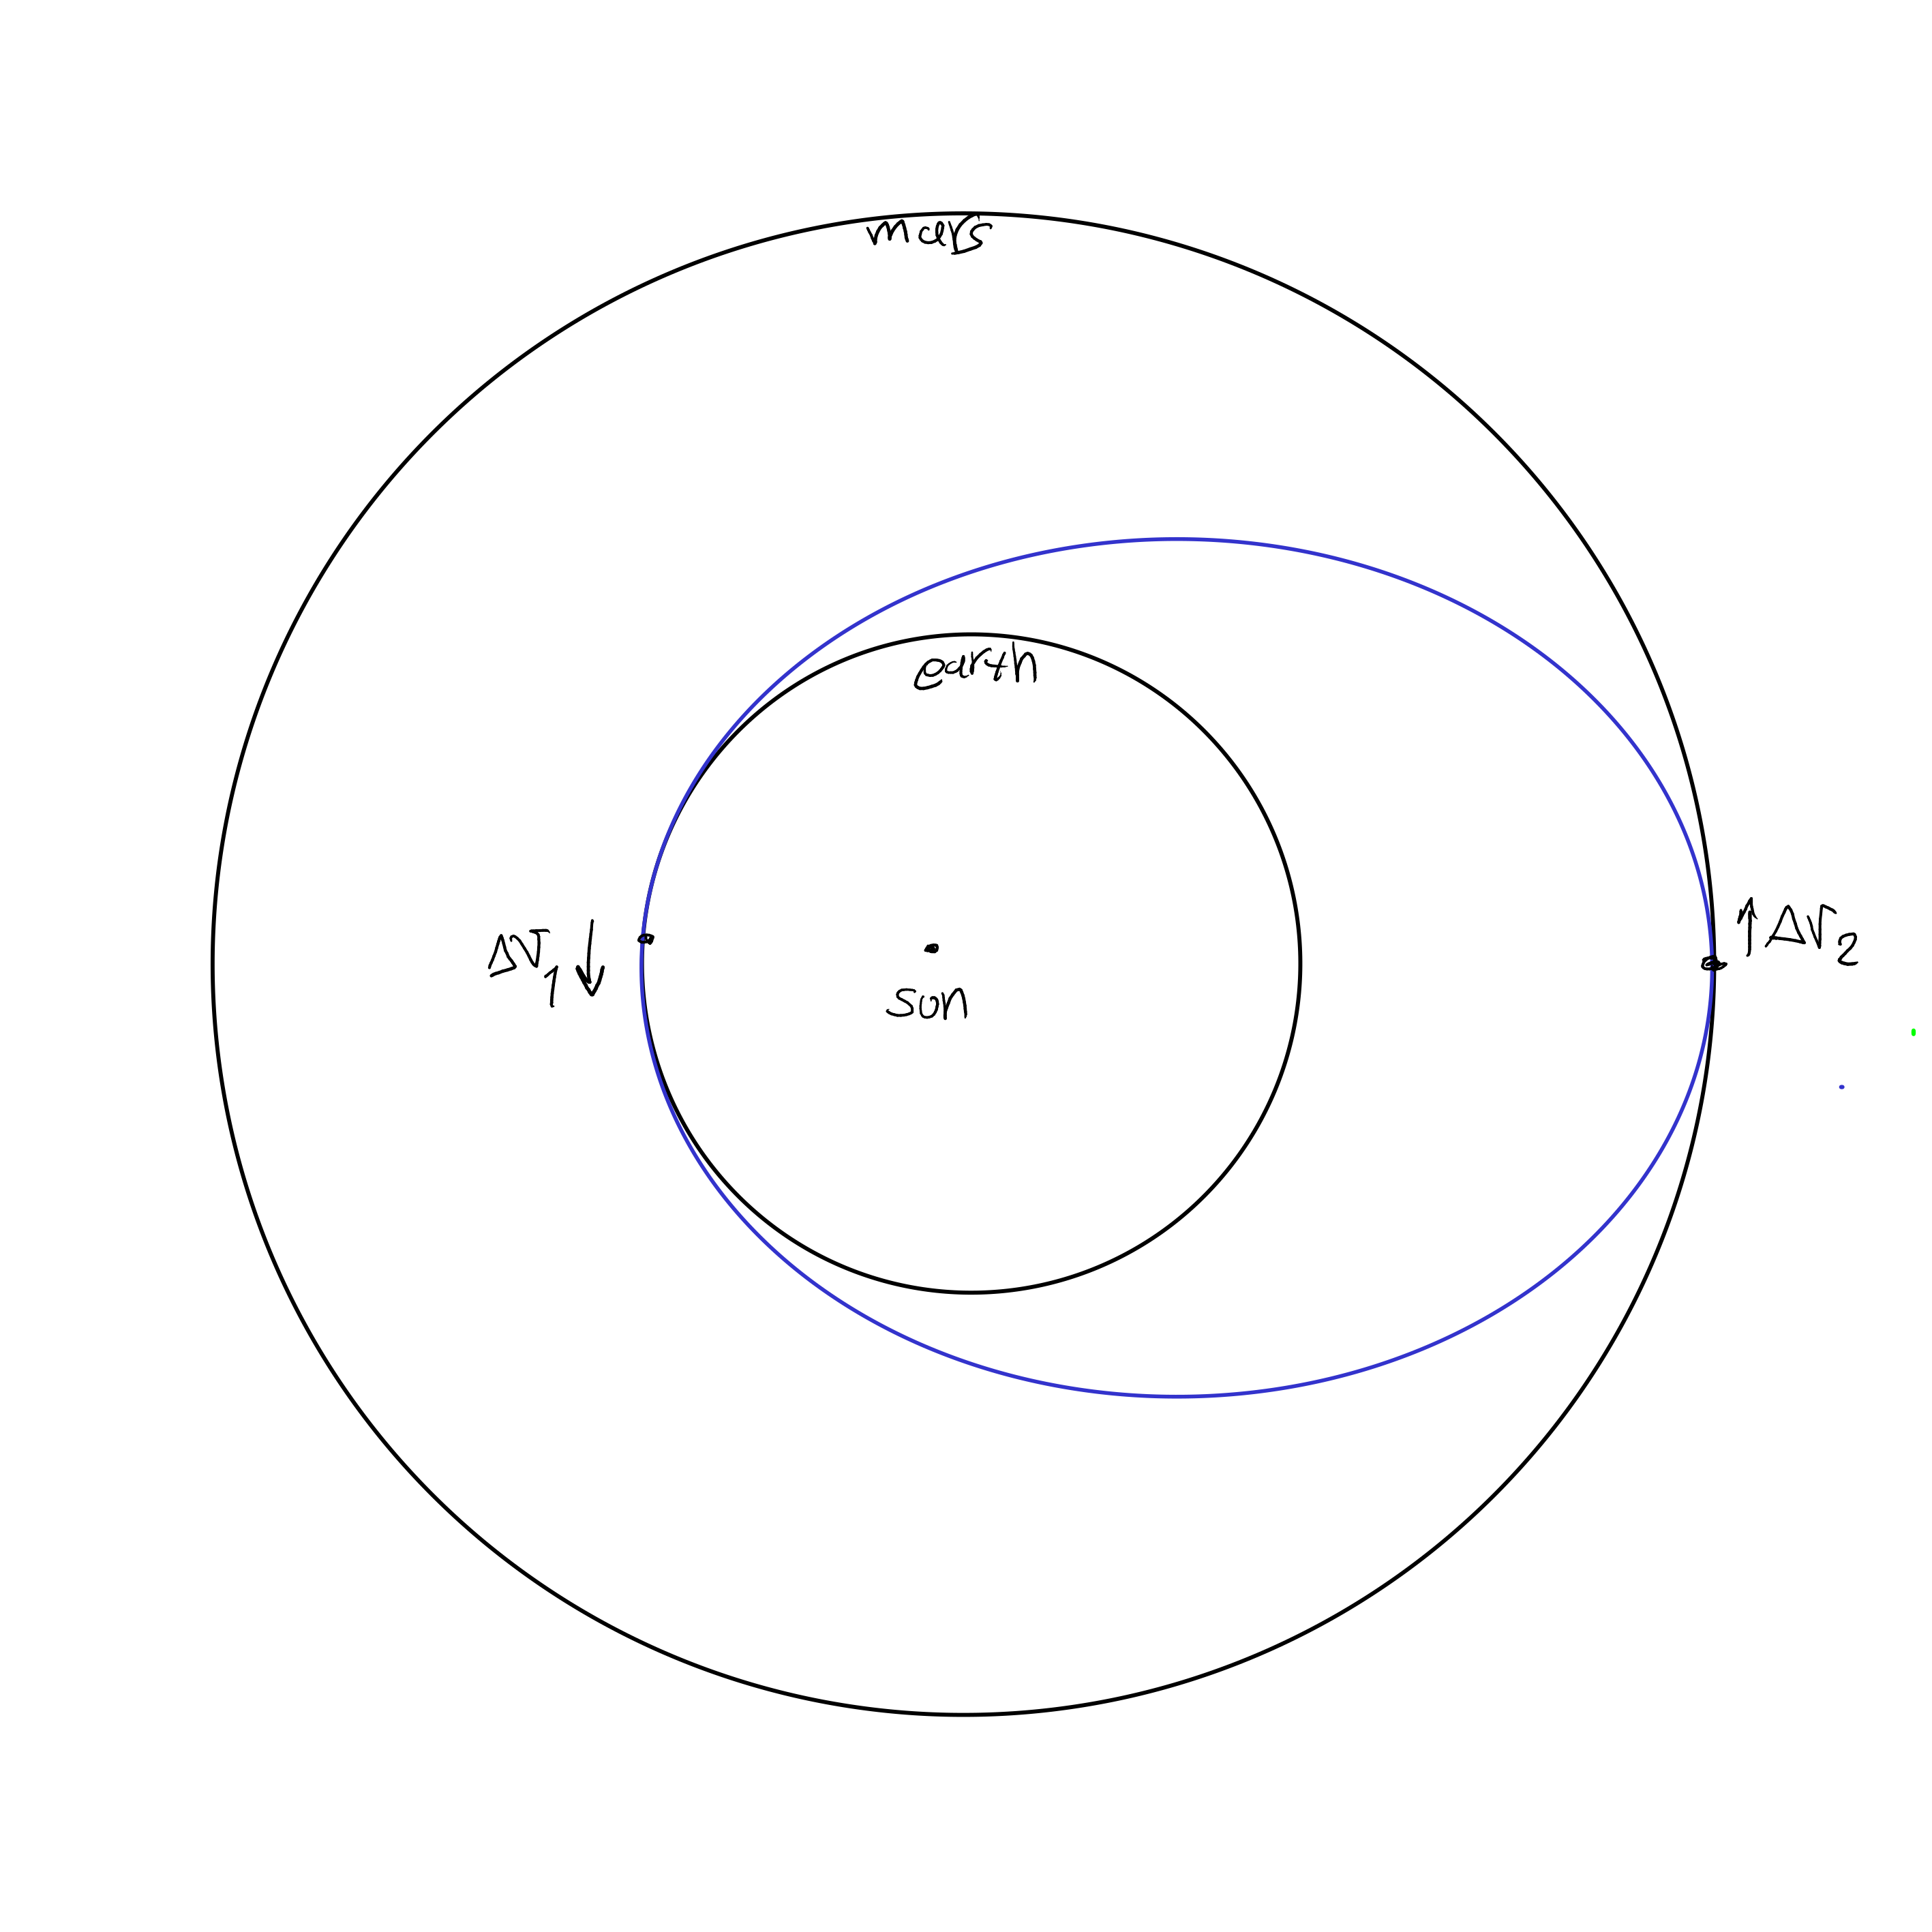
\includegraphics[width=\textwidth*8/9]{../results/hohman.png}
	
	\begin{align}
	a &= \frac{1 + 1.5}{2} = 1.25 AU \\
	e &= \frac{1.5 - 1}{1.5 + 1} = 0.2 \\
	v_p &= \sqrt{\frac{GM}{a}\left (\frac{1+e}{1-e}\right)} = 32668 \frac{m}{s} \\
	v_E &= \sqrt{\frac{GM}{r_E}} = 29821 \frac{m}{s} \\
	\Delta v_1 &= v_p - v_E = 2846 \frac{m}{s}
	\end{align}
	نکته قابل توجه این است که این تغییر سرعت نسبی، بسیار از سرعت فرار زمین کمتر است. در واقع برای سرعت فرار زمین داریم:
	\begin{align}
	v_{\text{فرار}} = \sqrt{\frac{2GM_E}{R_E}} = 11174 \frac{m}{s}
	\end{align}
	پس نمی‌توانیم مستقیما از سطح زمین این انتقال مداری را انجام دهیم. برای این کار از "مدار پارک" استفاده می‌کنیم.
	
	\section*{مدار پارک}
	در بسیاری از ماموریت های فضایی، قبل از ورود به مدار میان سیاره ای، فضاپیما وارد مداری به نام مدار پارک می‌شود. در ادامه، فضاپیما با یک مدار هذلولوی از مدار پارک خارج شده تا جایی که گرانش زمین در مسئله قابل چشم پوشی باشد. حال مانور هوهمان به طریقی که عقبتر گفته شد قابل انجام است. شکل تقریبی این مدار و محاسبات این مدار در ادامه آمده است (مسیر از سطح زمین به مدار پارک مشابه مدار هوهمان است و نقطه پرتاب در حضیض بیضی است):
	
	\includegraphics[width=\textwidth*8/9]{../results/park.png}
	
	\begin{align}
	R_{park} &= 4.22 \cross 10^6 m\\
	a &= \frac{R_{park} + R_E}{2} = 2.429 \cross 10^7 m\\
	e &= \frac{R_{park} - R_E}{R_{park} + R_E} = 0.737 \\
	\Delta \tilde{v_1} &=\tilde{v_p} - 0 = 10408 \frac{m}{s} \\
	\Delta \tilde{v_2} &= \sqrt{\frac{GM_E}{R_{park}}} - \tilde{v_a} = 1576 \frac{m}{s} \\
	\frac{\Delta E}{m} &= \frac{1}{2} (\Delta \tilde{v_1}^2 + \Delta \tilde{v_2}^2) = 5.541\cross 10^7 \frac{J}{Kg}
	\end{align}
	حال از مدار پارک تغییر سرعت مدار هوهمان را اعمال می‌کنیم(به کمک مدار هذلولی):
	\begin{align}
	\frac{E}{m} &= \frac{1}{2}(\tilde{v_1}^2 - \frac{GM_E}{R_{park}}) = \frac{1}{2} (v_p - v_E)^2 \\
	\implies \tilde{v_1} &= 5193 \frac{m}{s} \\
	\frac{\Delta E}{m} &= \frac{1}{2} (\tilde{v_1} - v_{park})^2 = 2.25 \cross 10^6 \frac{J}{Kg}
	\end{align}
	در انتقال مداری از مدار هوهمان به مدار مریخ به طور مشابه برای انرژی داریم:
	\begin{equation}
	\frac{E}{m} = 2 \cross 10^{6} \frac{J}{Kg}
	\end{equation}
	برای جرم فضاپیما از تخمین 
	$1 \cross 10^{4} Kg$
	استفاده می‌کنیم که تخمین معقولی است. در این صورت برای انرژی کل داریم:
	\begin{equation}
	E_{tot} = 5.966 \cross 10^{11} J
	\end{equation}
	برای این مقدار انرژی، سوخت مورد نیاز به صورت تخمینی برابر 
	$2000 Kg$
	است. (این مقدار در مقایسه با سوخت پنج هزار کیلوگرمی فضاپیمای ویجر منطقی است)
	\section*{شبیه سازی}
	برای شبیه سازی مسئله، هر شی (شامل خورشید، سیارات و فضاپیما) به عنوان یک آبجکت در زبان پایتون ساخته می‌شود. نمونه یک آبجکت در ادامه آمده است: \\
	
	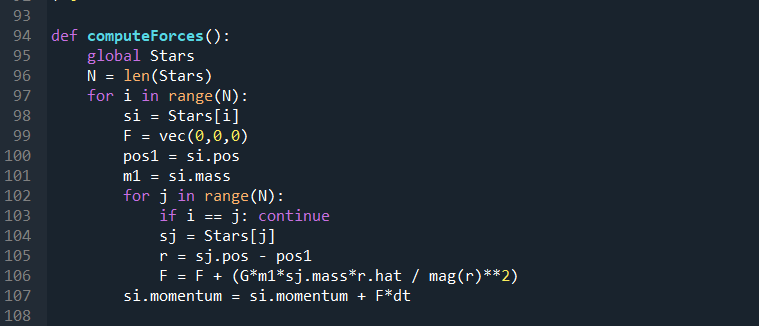
\includegraphics[width=\textwidth*8/9]{../results/code1}
	\\ \\
	در هر بازه زمانی کوچک تابع \lr{computeForces} نیروی های وارد بر هر جسم را برای محاسبه می‌کند و با کمک این نیرو، الگوریتم اویلر مسیر جسم را محاسبه می‌کند. (نیرو های مانور فضاپیما نیز در همین تابع قرار دارند): \\ \\
	\includegraphics[width=\textwidth*8/9]{../results/code2}
	\\ \\
	در ادامه نتایج شبیه سازی و نمودار های سرعت و مکان آورده شده: \\ \\
	
	\includegraphics[width=\textwidth*8/9]{../results/orbit1} \\
	\includegraphics[width=\textwidth*8/9]{../results/orbit2} \\
	\includegraphics[width=\textwidth*8/9]{../results/orbit3} \\
	\includegraphics[width=\textwidth*8/9]{../results/orbit4} \\
	\includegraphics[width=\textwidth*8/9]{../results/orbit5} \\
	\includegraphics[width=\textwidth*8/9]{../results/orbit6} \\ \\
	\includegraphics[width=\textwidth*8/9]{../results/graph1} \\
	\includegraphics[width=\textwidth*8/9]{../results/graph2} \\
	\includegraphics[width=\textwidth*8/9]{../results/graph3} \\ \\
	
	\section*{جمع بندی}
	طبق شبیه سازی، این سفر ۲۳۰ روز به طول می‌انجامد. این مقدار کمی از نیم دوره تناوب مدار هوهمان کمتر است که این تفاوت به علت تاثیر گرانشی مریخ است. همچنین زمان مناسب برای سفر مجدد دو سال و ۶۰ روز است. همچنین مشخصات مدار نهایی فضاپیما در ادامه آورده شده:
	\begin{align}
	0.9267 &= \text{خروج از مرکز} \\
	2.83 \cross 10^{8} m &= \text{نیم‌ قطر اول} \\
	\text{۵۳ روز و ۲۸ دقیقه} &= \text{دوره تناوب}
	\end{align} 
\end{document}
